\chapter{Project Description}
\lhead{ \thechapter \space Requirements Analysis}
\label{ch:requirements_analysis}
This chapter provides general information regarding the project, and can be considered an introductory chapter of the analysis done. Included is information about stakeholders, the scope, information about the drone, the risks, and a justification. 

\section{Stakeholders \& Affiliates}
Within this project, there are 3 groups of stakeholders: The student, Seacon Logistics, and \gls{FHTenL}. The latter 2 groups shall throughout this document be referred to as either "Seacon" or "the company", and "Fontys" or "the university", respectively. The table below lists individual stakeholders, to which group they belong to, and what their roles are.

\begin{table}[h]
	\centering
	\resizebox{\textwidth}{!}{%
		\begin{tabular}{|l|l|l|l|l|}
			\hline
			\textbf{Name} & \textbf{Company/Institute} & \textbf{Role} & \textbf{RACI Role} & \textbf{Email} \\ \hline
			Tristan van Vegchel & Fontys/Seacon Logistics & Student/Developer & Responsible & Tristan@vanvegchel.eu \\
			Sander Bruinsma & Fontys & Tutor & Informed & S.bruinsma@fontys.nl \\
			Geert Monsieur & Fontys & Examiner & Informed & G.monsieur@fontys.nl \\
			Kai-Arne Reiter & Seacon Logistics & Company Supervisor & Consulted, Informed & Kreiter@seaconlogistics.com \\
			Mark Vromans & Seacon Logistics & Manager Engineering \& IT & Accountable, Informed & Mvromans@seaconlogistics.com \\
			Wilfried Beerens & Seacon Logistics & Manager Shared Services Center & Informed & Wbeerens@seaconlogistics.com \\
			Fred Lemmen & Seacon Logistics & Senior Application Specialist & Consulted & flemmen@seaconlogistics.com \\ \hline
		\end{tabular}%
	}
	\caption{List of stakeholders with their respective roles.}
	\label{tab:stakeholders}
\end{table}
Stakeholders, aside from their regular roles, also have a \gls{RACI} role assigned to them. For a description of the roles, please refer to table \ref{tab:raci_matrix}.
\begin{table}[h]
	\centering
	\resizebox{\textwidth}{!}{%
		\begin{tabular}{l|l|l}
			Abbreviation letter & Definition  & Description \\ \hline
			\textbf{R}          & Responsible & Who is assigned to work on this task?           \\
			\textbf{A}          & Accountable & Who has the authority to take decisions and who will be held accountable for the consequences?           \\
			\textbf{C}          & Consulted   & Who are considered stakeholders and who can provide more information about this task?           \\
			\textbf{I}          & Informed    & Whose work depends on this task and who has to kept updated about the progress?          
		\end{tabular}%
	}
	\caption{Descriptions of the RACI matrix roles.}
	\label{tab:raci_matrix}
\end{table}
\pagebreak
\section{Minimal Product}
The minimal product is considered to be the bare minimal functionality for a project to be considered successful. In the case of this project that is to be able to supply a drone with a solution that lets it move along one side of the rack, while preventing itself from colliding with objects. When talking about objects, the following things are generally meant:
\begin{itemize}
	\itemsep0em
	\item Pallets
	\item Racks
	\item Forklifts
	\item People
	\item Drones
\end{itemize}
\noindent
As Seacon eventually wants to make use of disposable drones, it is essential for the drone to have as few sensors as possible. Unless it is proven impossible with just the use of a monocular camera-equipped drone, however, the use of additional sensors is advised against.

\section{Drone Description}
This project will make use of the DJI Tello drone (figure \ref{fig:tello}). The drone has been made available by Seacon, and was chosen based on its price, sturdiness, API availability, and functionality. As Seacon wants to make use of disposable drones in the future, the amount of sensors should be kept to a minimum. The Tello drone is equipped with a front-facing color 720p camera, a vision positioning system that makes use of an infrared sensor pointing to the ground below it, and a collision detection system that instantly stops the propellers upon contact \citep{tello}.

\begin{figure}[h]
	\centering
	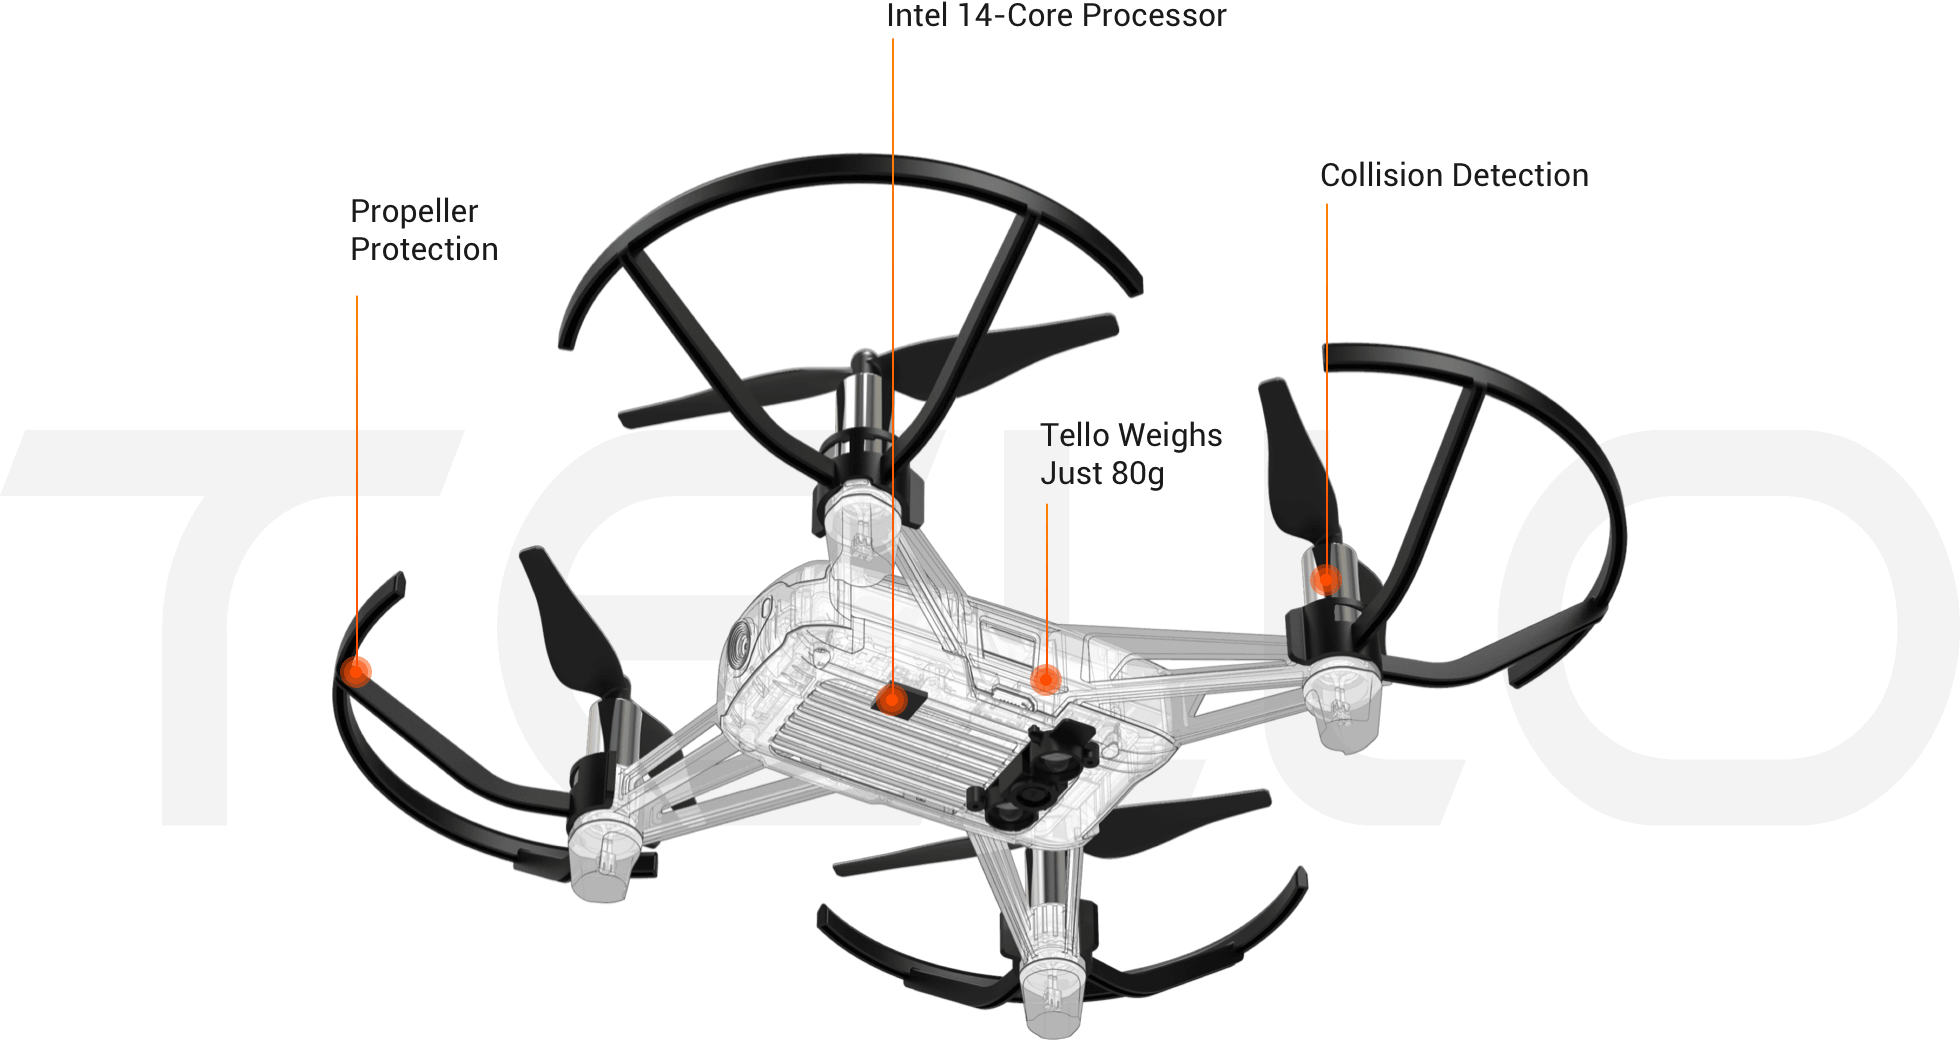
\includegraphics[width=0.75\linewidth]{img/tello}
	\label{fig:tello}
	\caption[Image of the Tello drone.]{Image of the DJI Tello drone. Source: \citep{tello}}
\end{figure}

\pagebreak
\section{Time Scope}
This project has been carried out over a period of 5 months, starting from September 2019 until January 2020. Within this period a couple of milestone dates exist, which were defined by \gls{FHTenL}. These dates can be found in the table below:
\begin{table}[h]
	\centering
	\begin{tabular}{|l|l|}
		\hline
		\textbf{Deliverable} & \textbf{Deadline} \\ \hline
		Project Plan & 27/09/2019 \\
		Midterm Report & 21/10/2019 \\
		Midterm Presentation & 11/11/2019 \\
		Thesis Report & 13/01/2020 \\
		Final Presentation & 27/01/2020 \\ \hline
	\end{tabular}
	\caption{List of school deadlines.}
	\label{tab:deadlines}
\end{table}

\section{Risk Analysis}
In order to minimize damage caused by risks, a risk analysis has been carried out. This has resulted in the creation of a risk matrix, which, due to its size, has been moved to appendix \ref{app:risks}. The matrix contains a list of risks, the consequences, and its scores based on the likelihood and impact. It also contains a mitigation plan to reduce its score, together with a set of new scores based on the effect of the mitigation.

\section{Project Justification}
\begin{table}[h]
	\centering
	\resizebox{\textwidth}{!}{%
		\begin{tabular}{l|l}
			\textbf{Description} & \textbf{Estimated values} \\ \hline
			Amount of locations & 80000 \\
			Times counted & 3 \\
			2nd and 3rd counts & 1000 \\ \hline
			Total locations ((amount of locations + 2nd and 3rd counts) * times counted) & 243000 \\
			Average time (seconds) per location & 30 \\ \hline
			Total work hours per annum & 2025 \\
			Amount of employees & 2 \\
			Warehouse employee cost per hour (euros) & 20 \\ \hline
			\textbf{Total costs warehouse employees (euros)} & 81000 \\
			\textbf{Total costs (including office employees and forklift costs) (euros)} & 95000
		\end{tabular}%
	}
	\caption[Estimated annual costs of cycle counts for 2020]{Estimated annual costs of cycle counts for 2020, based on a 30 second average per location.}
	\label{tab:costs}
\end{table}
One might wonder why instead of improving inventory control processes not improve picking and storing processes. While it is true that, in the absolute ideal case where storing and picking happens flawlessly, maintenance processes such as \gls{cycle_count}s wouldn't need frequent occurrences. However, considering that humans are involved in these processes it is safe to assume human mistakes will happen. Moreover, as warehouse employees are getting scarcer, the standard for hiring new employees keeps lowering, which results in more mistakes happening.
\\\\
According to \gls{CBS}, the working sector for transport and storage had roughly 8000 work-related injuries with a 4+ days absence occur in 2017. This ranks this sector the 4th highest sector with the most reported 4+ days absence work-related injuries, and the second-highest sector when looking at the percentage of employees sustaining injuries in comparison to the total number of employees in that sector \citep{cbs}.
\\\\
As seen in table \ref{tab:costs}, the estimated costs for 2020 is roughly \euro95000, of which \euro81000 goes to employees performing the cycle counts. Using drones could reduce the number of hours of those employees significantly, and thus reduce the largest cost in the whole cycle count process. It is important to note that the numbers used in this table have been altered slightly for privacy reasons.

